% Data flow diagram
% Author: David Fokkema
\documentclass{article}
\usepackage{tikz}
\usetikzlibrary{shapes,arrows}
\usepackage{pdflscape}
\usepackage[papersize={7.5cm, 4.7cm}, text={7.5cm, 4.7cm}]{geometry}
\usetikzlibrary{decorations.text}
\usepackage{xcolor}
% \selectcolormodel{gray}

\begin{document}
\thispagestyle{empty}
%\begin{landscape}
\begin{center}
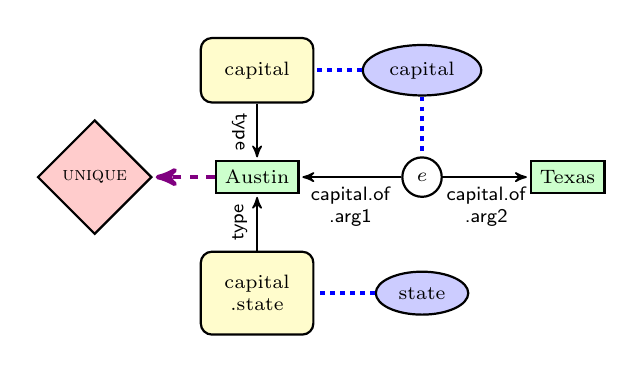
\begin{tikzpicture}[
  font=\sffamily,
  every matrix/.style={ampersand replacement=\&,column sep=0.6cm,row
sep=0.2cm,font=\scriptsize},
  entity/.style={draw,thick,rectangle,fill=green!20},
  word/.style={draw,thick,ellipse,fill=blue!20},
  mediator/.style={draw,thick,circle},
  entityType/.style={draw,thick,rounded corners,fill=yellow!20,inner sep=.3cm},
  mathType/.style={draw,thick,diamond,fill=red!20,font=\sc\scriptsize},
  mediatorToEntity/.style={->,>=stealth',shorten
>=1pt,semithick,black,sloped,above,font=\sffamily\scriptsize},
  typeToEntity/.style={->,>=stealth',shorten
>=1pt,semithick,black,sloped,above,font=\sffamily\scriptsize},
  wordToEntity/.style={-,>=stealth',shorten >=1pt,ultra
thick,dotted,blue,sloped,above,font=\sffamily\scriptsize},
  entityToMath/.style={->,>=stealth',shorten >=1pt,ultra
thick,dashed,violet,sloped,above,font=\sffamily\scriptsize},
  every node/.style={align=center}]

  % Austin_1 is_2 the_3 state_4 capital_5 of_6 Texas_7
  
  % Position the nodes using a matrix layout
  \matrix{ 
    \& \node[entityType] (tCapital) {capital}; \& \node[word]
(wCapital)
{capital}; \& \\
    \node[mathType] (mUniq) {unique};  \& \node[entity] (eAustin) {Austin};
\& \node[mediator] (mCapital) {$e$}; \& \node[entity] (eTexas) {Texas}; \\
   \& \node[entityType] (tState)
{capital\\.state}; \& \node[word] (wState) {state}; \& \\ 
  };
 
  % words to entities
  % \draw [wordToEntity] (wAustin) edge node {}  (eAustin);
  % \draw [wordToEntity] (wTexas) edge node {}  (eTexas);
  % words to types
  \draw [wordToEntity] (wCapital) edge node {}  (tCapital);
  \draw [wordToEntity] (wState) edge node {}  (tState);
  
  % type to entity
  \draw [typeToEntity][below] (tCapital) edge node {type}  (eAustin);
  \draw [typeToEntity] (tState) edge node {type}  (eAustin);
  
  % event word to mediators
  \draw [wordToEntity] (wCapital) edge node {}  (mCapital);
  
  % mediator to entities
  \draw [mediatorToEntity][below] (mCapital) edge node {capital.of\\.arg1}  (eAustin);
  \draw [mediatorToEntity][below] (mCapital) edge node {capital.of\\.arg2}  (eTexas);
   
   \draw [entityToMath] (eAustin) edge node {}  (mUniq);
   % \draw [wordToEntity] (wAustin) edge node {}  (mUniq);
  
\end{tikzpicture} 
\scriptsize \scriptsize
$\textsc{unique}(\mathrm{Austin}) \wedge \mbox{capital}(\mathrm{Austin})
\wedge \mbox{capital.state}(\mathrm{Austin}) \wedge
   \mbox{capital.of.arg1}(e,
\mathrm{Austin}) \wedge \mbox{capital.of.arg2}(e, \mathrm{Texas})$
\end{center}

\end{document}